
Для минимизации булевых функций воспользуемся картами Карно. 

\begin{center}
  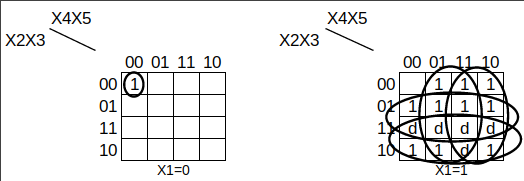
\includegraphics[width=\linewidth]{imgs/part2/carno_C1.png}
\end{center}
$C_{min}(C1)=\{00000, 1X1XX, 11XXX, 1XXX1, 1XX1X\} \\
S^a=14, S^b=19 \\
C_1 = \nx{1}\nx{2}\nx{3}\nx{4}\nx{5}\vee\x{1}\x{3}\vee\x{1}\x{2}\vee\x{1}\x{5}\vee\x{1}\x{4} \\
S^{C_1}_Q = 18
$

\begin{center}
  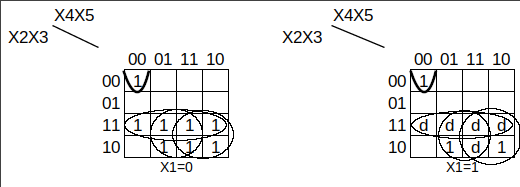
\includegraphics[width=\linewidth]{imgs/part2/carno_C2.png}
\end{center}
$C_{min}(C2)=\{X0000, X11XX, XX1X1, X1X1X\} \\
S^a=10, S^b=14 \\
C_2 = \nx{2}\nx{3}\nx{4}\nx{5}\vee\x{2}\x{3}\vee\x{3}\x{5}\vee\x{2}\x{4} \\
S^{C_2}_Q = 14
$

\begin{center}
  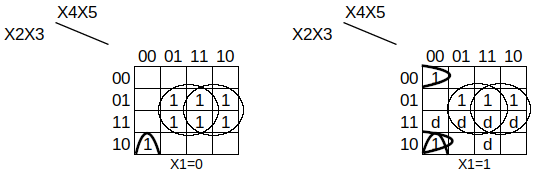
\includegraphics[width=\linewidth]{imgs/part2/carno_C3.png}
\end{center}
$C_{min}(C3)=\{1X000, X1000, XX1X1, XX11X\} \\
S^a=13, S^b=17 \\
C_3 = \x{1}\nx{3}\nx{4}\nx{5}\vee\x{2}\nx{3}\nx{4}\nx{5}\vee\x{3}\x{5}\vee\x{3}\x{4} \\
S^{C_3}_Q = 16
$

\begin{center}
  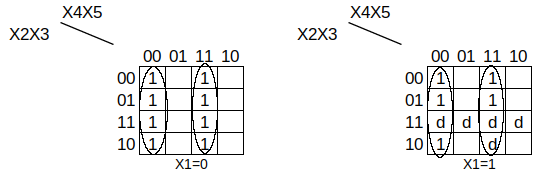
\includegraphics[width=\linewidth]{imgs/part2/carno_C4.png}
\end{center}
$C_{min}(C4)=\{XXX00, XXX11\} \\
S^a=4, S^b=6 \\
C_4 = \nx{4}\nx{5}\vee\x{4}\x{5} \\
S^{C_4}_Q = 6
$

\begin{center}
  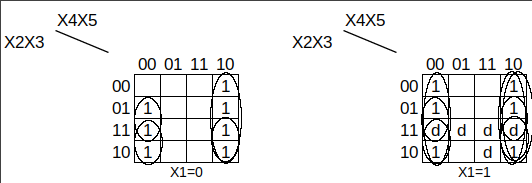
\includegraphics[width=\linewidth]{imgs/part2/carno_C5.png}
\end{center}
$C_{min}(C5)=\{XXX10, 1XXX0, X1XX0, XX1X0\} \\
S^a=8, S^b=12 \\
C_5 = \x{4}\nx{5}\vee\x{1}\nx{5}\vee\x{2}\nx{5}\vee\x{3}\nx{5} \\
S^{C_5}_Q = 12 \\
$
При реализации схемы в виде пяти независимых подсхем ее цена $S_Q=66$. \\